\chapter{Les propietats i el comportament dels gasos}

L'estudi dels gasos és fonamental per a comprendre el comportament de la matèria en estat gasós. Aquests conceptes són claus tant en la química moderna com en l'aplicació industrial. Les lleis dels gasos proporcionen una base per descriure el comportament macroscòpic dels gasos en funció de la temperatura, el volum i la pressió.



\section{Les lleis dels gasos}
En general, el volum d'un gas està determinat per la seva temperatura i la pressió que suporta. Existeix una relació matemàtica entre aquests paràmetres, que s'expressa com l'\textbf{equació d'estat}:
\begin{equation}
V = V(T, P, n),
\end{equation}
on $V$ és el volum, $T$ és la temperatura, $P$ la pressió, i $n$ el nombre de mols del material. Es tracta d'una equació que pot ser molt complexa i específica per a líquids i sòlids, però en el cas dels gasos tots ells tenen un comportament molt similar. Això és degut a que en l'estat gas, les molècules són mes independents entre elles i, per tant, la seva naturalesa molecular no afecta substancialment al comportament del tot.

\begin{mybox}[title=De partícules i mols de partícules]
    El mol és la unitat bàsica del Sistema Internacional per mesurar la quantitat de substància, i s'utilitza per comptar partícules com àtoms, molècules o ions. Un mol conté exactament \(N_0=6,022 \times 10^{23}\) entitats elementals, un valor conegut com el nombre d'Avogadro. Aquesta constant permet connectar les dimensions microscòpiques (com la massa i el nombre de partícules) amb mesures macroscòpiques utilitzades en els experiments químics. Per exemple, un mol d'àtoms de carboni-12 (que representarem per \isotope*{12,C}, a partir d'ara) té una massa de 12 grams, facilitant així la relació entre l'estructura atòmica i la pràctica de la química.
\end{mybox}
    
\subsection{Pressió i força}

Un dispositiu típic per mesurar la pressió és el baròmetre, que utilitza una columna de mercuri per determinar la pressió atmosfèrica. 

\begin{figure}[h]
    \centering
    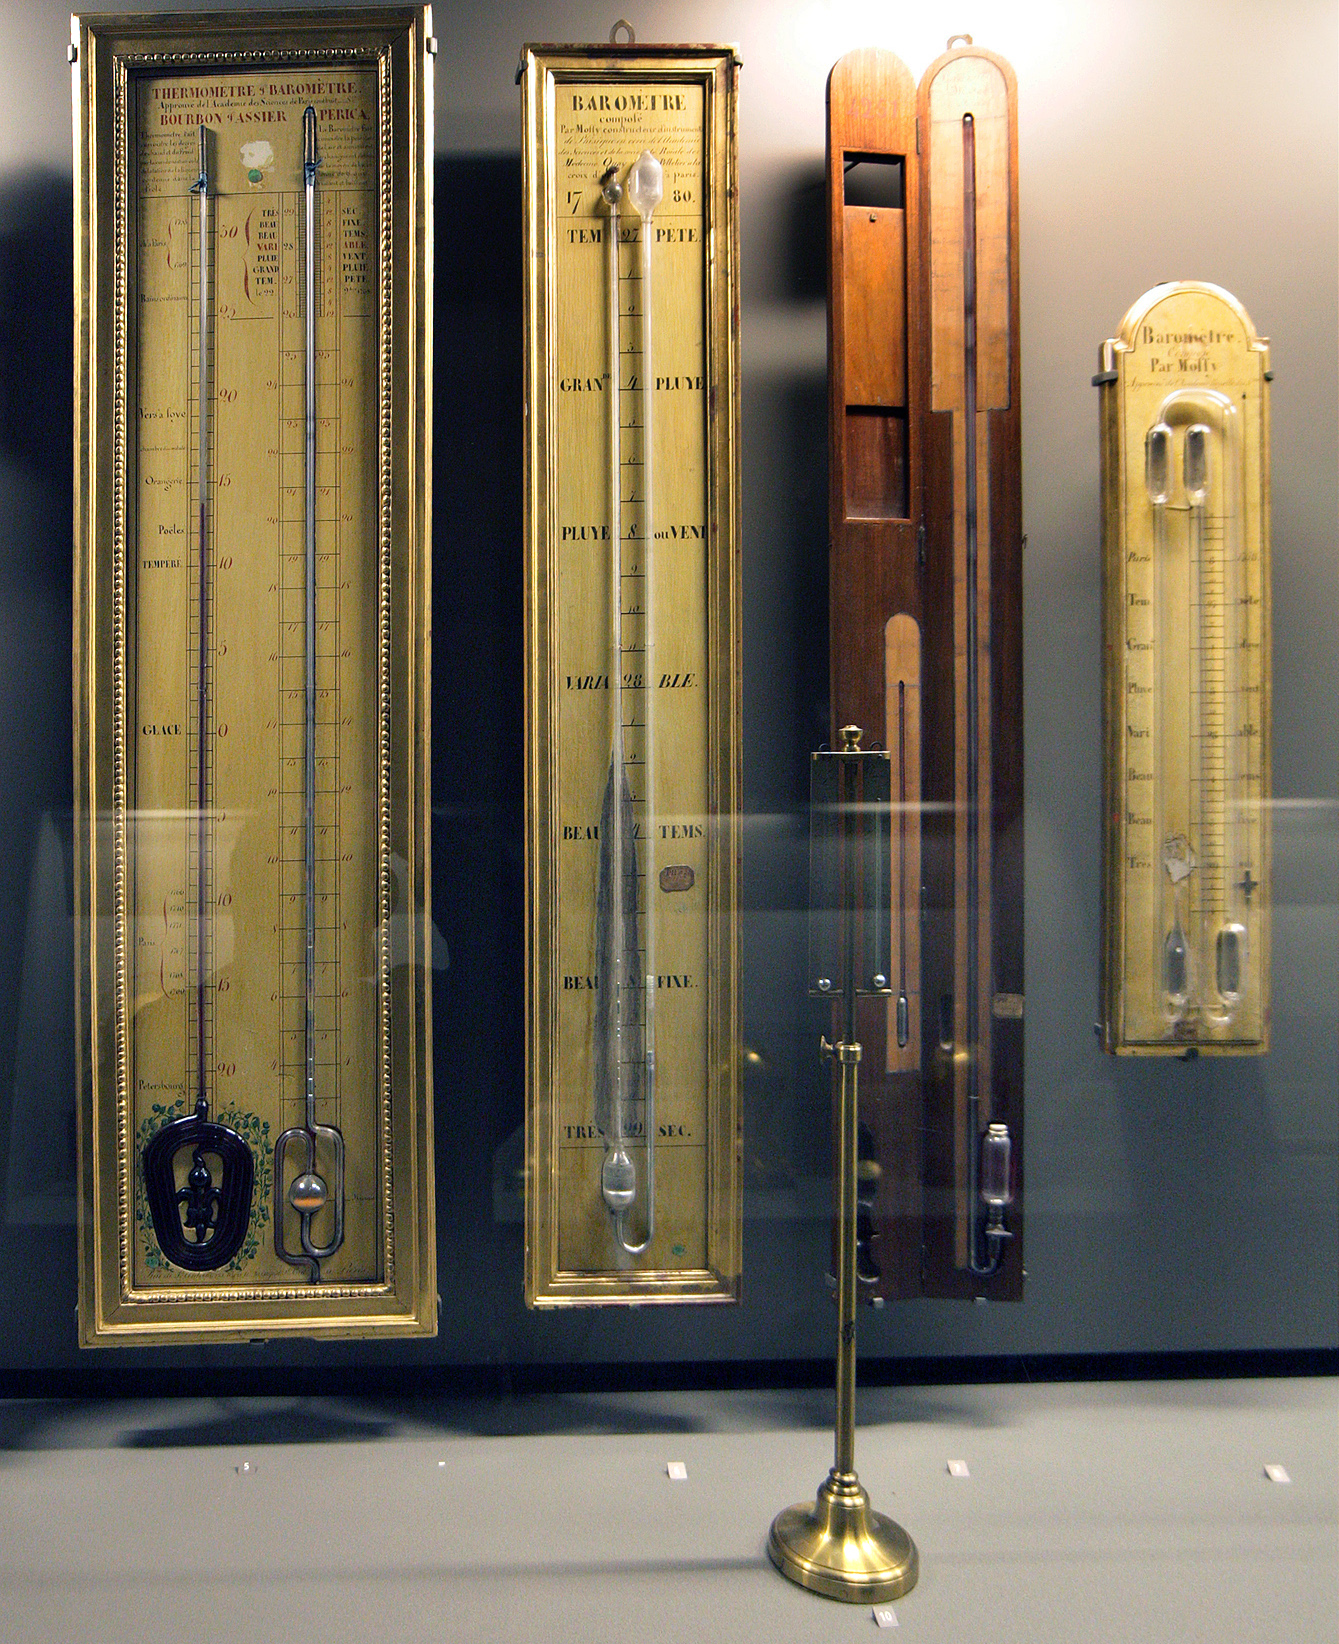
\includegraphics[width=0.33\textwidth]{Old-barometers.jpg}
    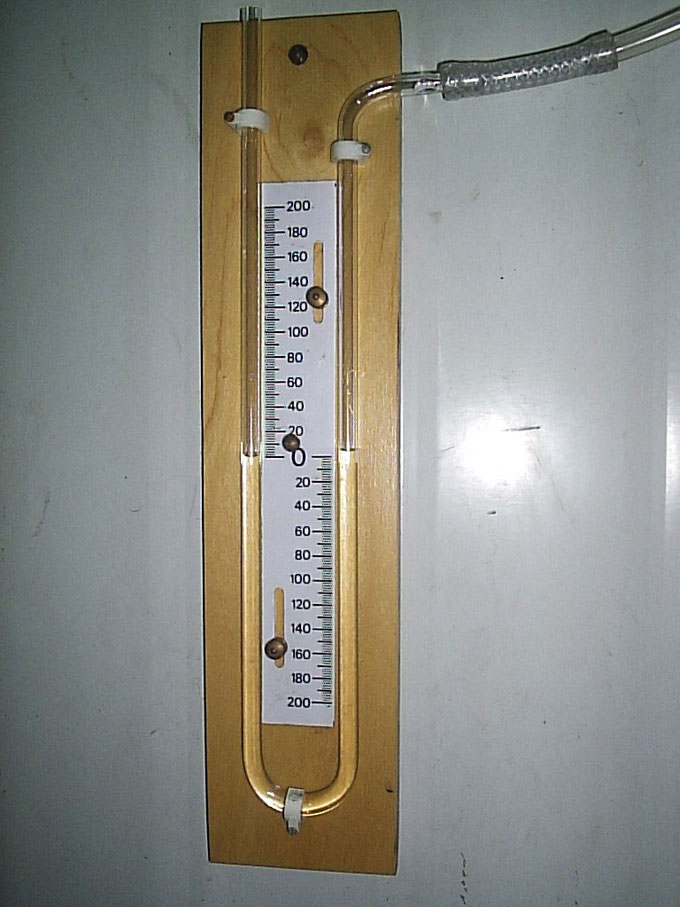
\includegraphics[width=0.33\textwidth]{Manometre.png}
    \caption[Baròmetre i Manòmetre diferencial]{El baròmetre (esquerra) utilitza una columna de mercuri per determinar la pressió atmosfèrica. Un manòmetre diferencial (dreta) mesura la diferència entre les pressions externes i d'un determinat gas.}
    \label{fig:Manometre}
    \end{figure}

La pressió és definida com la força per unitat d'àrea que un gas exerceix sobre les parets del recipient que el conté. S'expressa comunament en unitats com pascals (\si\pascal) o atmosferes (\si\atm). Matemàticament:
\begin{equation}
\text{Pressió} = \frac{\text{Força}}{\text{Àrea}} = \frac{\text{massa} \times \text{acceleració}}{\text{Àrea}} = \frac{\text{massa} \times \text{acceleració}}{\text{Volum / alçada}} 
\end{equation}
Per tant, la pressió es calcula com:
\begin{equation}
P = \rho \cdot g \cdot h,
\end{equation}
on $\rho$ és la densitat, $g$ l'acceleració gravitatòria i $h$ l'alçada.

Calculem ara què és una atmosfera quan s'expressa en funció de força per àrea unitaria. Considerem una columna de mercuri amb una alçada de 760 mm. Sabem que la densitat del mercuri és $13.6 \cdot 10^3 \si{\kg\per\meter\tothe{3}}$ i l'acceleració gravitatòria és $9.8 \si{\meter\per\square\second}$.  Considerem un tub baromètric la superfície de secció transversal del qual és 1 \si{\square\cm}. Aleshores, la força que exerceix la columna de mercuri sobre aquesta superfície és igual a la massa del mercuri que es troba al tub, multiplicada per l'acceleració deguda a la gravetat. A la vegada, la massa del mercuri que està en el tub és el volum del mercuri multiplicat per la seva densitat a $0^{\circ}\text{C}$. Així doncs, es té:

\[
\text{força} = 
\]
\[
= \text{densitat del Hg} \times \text{alçada} \times \text{àrea} \times \text{acceleració}
\]
\[
= 13,59 \, \frac{\si\g}{\si{\cubic\cm}} \times 76,00 \, \si{\cm} \times 1,000 \, \si{\square\cm} \times 980,7 \, \frac{\si{\cm}}{\si{\s}^2}
\]
\[
= 1,013 \times 10^6 \, \si\g \cdot \frac{\si\cm}{\si{\s}^2} = 10,13 \, \si\kg \cdot \frac{\si\m}{\si{\s^2}}
\]
\[
= 10,13 \si{\newton}.
\]

Aquesta és la força que exerceix una columna de mercuri de 760 mm d'alçada i d'1 $\text{cm}^2$ de superfície de secció transversal. Per tant, és també la força per unitat de superfície (un centímetre quadrat) que correspon a la pressió d'una atmosfera. Així, es té que:

\[
1 \, \si{\atm} = 760,0 \, \si\mmHg= 760 \,\si\torr
= 1,013 \times 10^6 \, \si{\dyn\per\square\cm} = 1,013 \times 10^5 \, \si{\newton\per\square\meter}.
\]

Els gasos es comporten segons certes lleis empíriques que han estat establertes experimentalment. Aquestes lleis condueixen finalment a la formulació de la llei dels gasos ideals.

\begin{mybox}[title=Quantitats intensives i extensives]
    Les propietats es poden classificar entre extensives (m, V, ...) o intensives (T, P, capacitat calorífica ...), segons depenguin de la quantitat de substància o no. La raó entre dues propietats extensives és sempre intensiva: $\delta = \frac{m}{V}$; $\nu = \frac{V}{m}$. Només necessitem dues propietats intensives per determinar l'estat d'un gas ($P$ i $T$) i, per tant, amb tres variables intensives podem construir una equació d'estat: 
    \[F(P,V_{\rm m},T)=0\]
    
    La mesura d'una propietat per mol sanomena valor molar d'aquesta variable. Per exemple $V_{\rm m} = \frac{V}{n}$. 
\end{mybox}

\begin{exr}
    Calcular el volum molar d'un gas ideal a condicions normals (1 atm i 0\si\degreeCelsius).
    \end{exr}
\subsection{Llei de Boyle}

Robert Boyle (1627-1691) va notar, fent servir un manometre com el de la Figura \ref{fig:Manometre}, que existia una determinada llei de proporcionalitat entre la pressió exercida sobre un gas i el volum d'aquest
\begin{figure}[h]
\centering
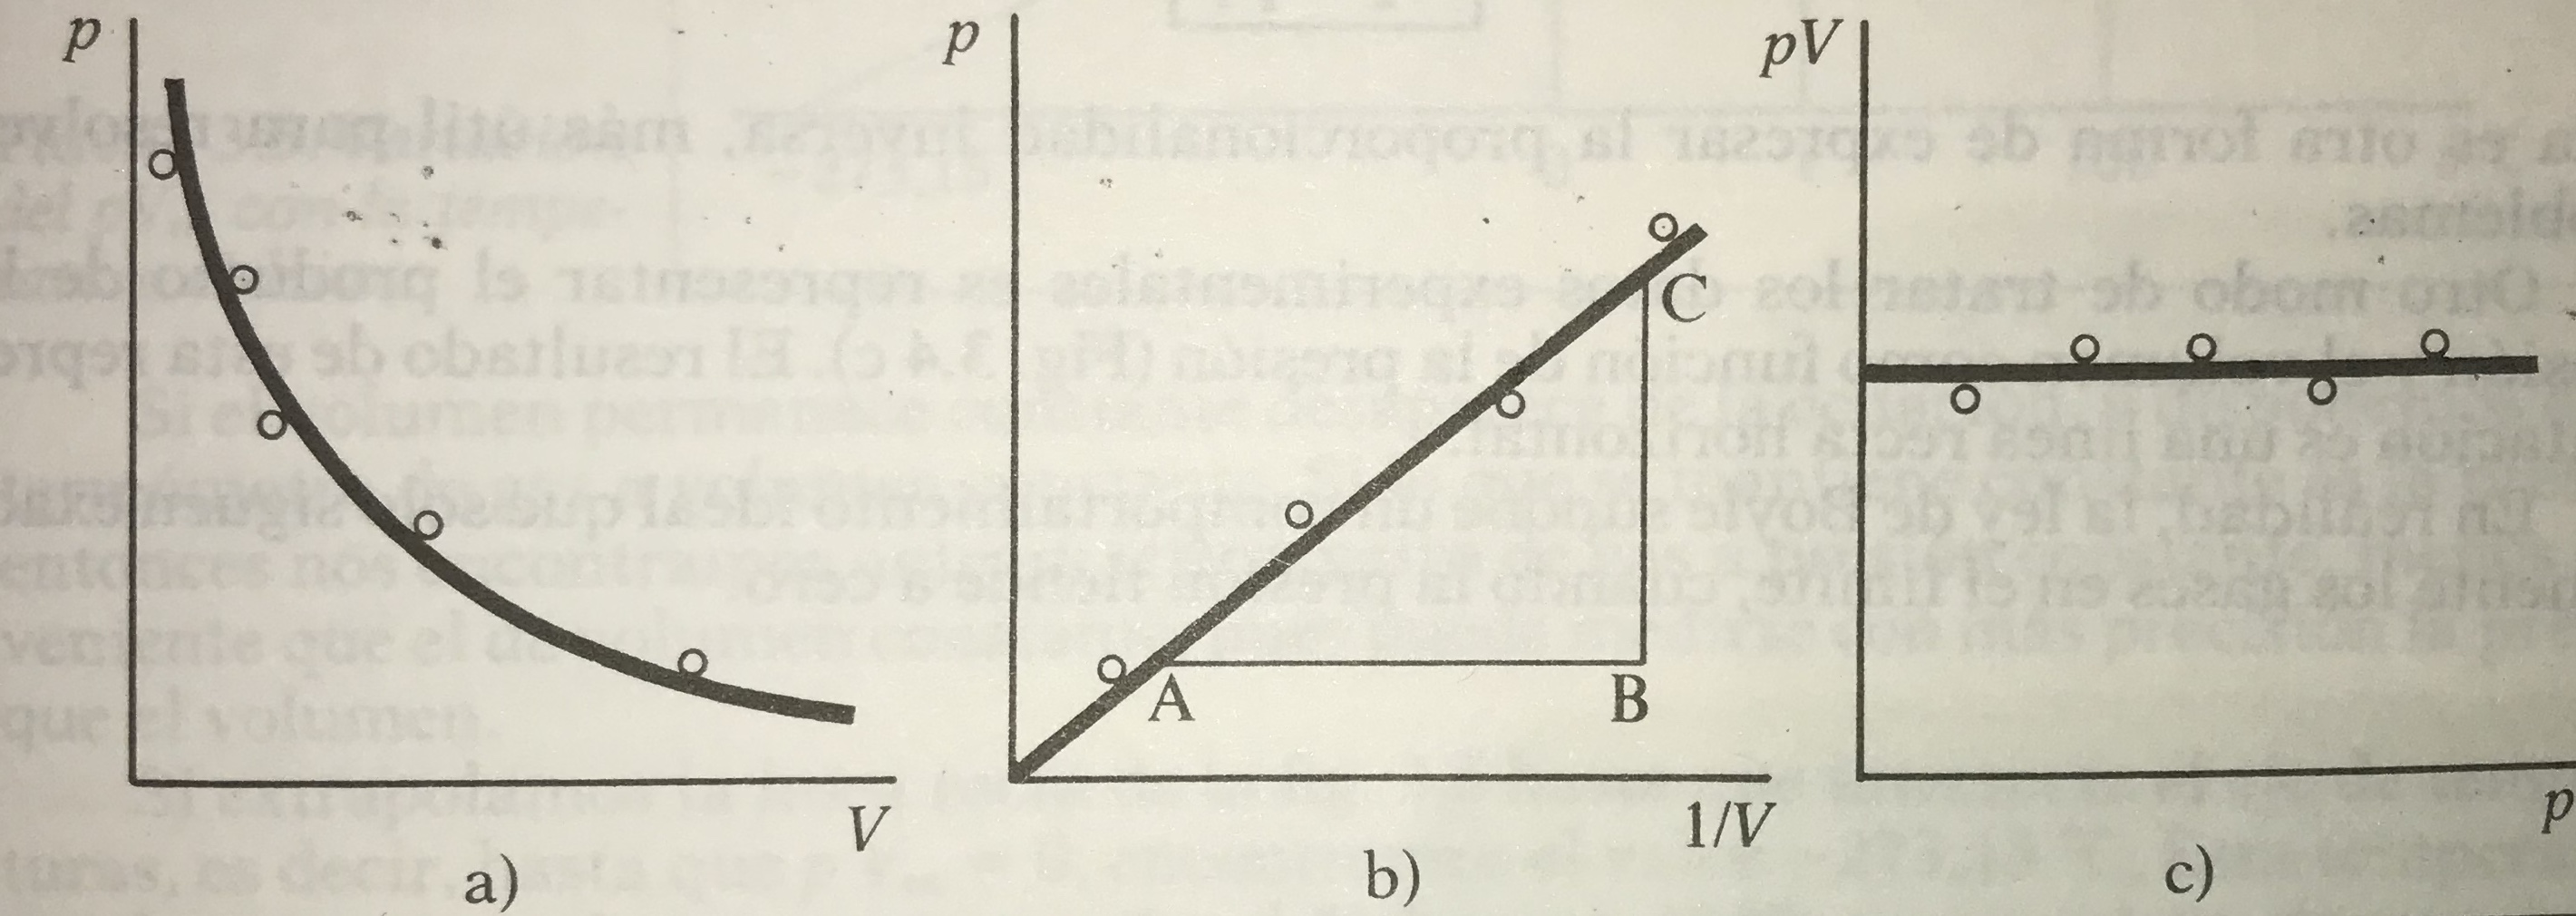
\includegraphics[scale=0.10]{Boyle.png}
\caption{Experiment de Boyle i llei de proporcionalitat entre la pressió exercida sobre un gas i el seu volum.}
\label{fig:Boyle}
\end{figure}
Va descobrir que el producte entre el volum i la pressió és una constant, la qual cosa duu a que sota dues condicions diferents de pressió els volums es comporten de la següent manera per al mateix gas a una temperatura donada:
\[
\frac{V_1}{V_2}=\frac{P_2}{P_1}
\]

Així, la pressió \( P \) d'un gas és inversament proporcional al seu volum \( V \):
\begin{equation}
    P V = \text{constant}
\end{equation}
On \( P \) s'expressa en \si{Pa} (pascals) i \( V \) en \si{m^3}.

\subsection{Llei de Charles}

Jacques Charles (1787) i posteriorment Gay-Lussac van trobar que per a una mateixa pressió, la relació $\frac{V_{100 \si\degreeCelsius}}{V_{0 \si\degreeCelsius}}$ era identica per a tots els gasos (1.376).

Això duu a extrapolar fàcilment el comportament dels gasos i determinar el zero absolut de temperatura segons el gràfic \ref{fig:zeroabsolut}. Lord Kelvin (1848) va proposar usar el punt d'intersecció del gràfic amb la línia de les abcisses com a origen d'una nova escala de temperatura: $T/\rm{K} = t/\si\degreeCelsius \rm{C} + 273.15$.\marginnote{en realitat s'usa 273.16, que és el punt triple de l'aigua, temperatura a la qual coexisteixen en equilibri aigua, gel i vapor en un recipient tancat}
\begin{figure}[h]
\centering
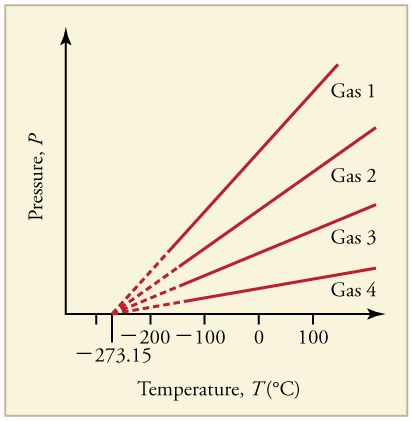
\includegraphics[scale=1.0]{zeroabsolut.png}
\caption{Gràfic del zero absolut a partir de la llei de Charles i Gay-Lussac.}
\label{fig:zeroabsolut}
\end{figure}

La llei de Charles afirma que, a pressió constant, el volum d'un gas és directament proporcional a la seva temperatura absoluta \( T \):
\begin{equation}
    \frac{V}{T} = \text{constant}
\end{equation}
On \( T \) es mesura en \si{K} (kelvins).

\subsection{Llei d'Amonton (o de Gay-Lussac)}
La llei de Gay-Lussac és una llei dels gasos que estableix que la pressió \( P \) exercida per un gas (d'una massa donada i mantingut a volum constant) varia directament amb la temperatura absoluta del gas:
\begin{equation}
    T \propto P \quad \text{o} \quad P = \text{constant} \times T
\end{equation}
En altres paraules, si un gas ideal està confinat en un recipient amb volum constant i s'incrementa la temperatura, la pressió augmentarà proporcionalment a la temperatura.

\begin{exr}
    Un conductor comprova la pressió dels pneumàtics pel matí aviat, quan la temperatura és de 15\si\degreeCelsius, i és de 1.3$\times$10$^5$ Pa. Al migdia la temperatura és 15 graus més elevada. Quina és la pressió dels pneumàtics ara?.
    \end{exr}

      
    \begin{exr}
        Dalt de l'Everest, la pressió atmosfèrica és de 0,33 atm i la temperatura de 50 sota zero. Quina és la densitat de l'aire si en CN és de 1.29\si{\gram\per\deci\meter\tothe{3}}?.
        \end{exr}
    

\subsection{Llei dels Gasos Ideals}
Combinant les tres lleis anteriors, obtenim la llei dels gasos ideals:
\begin{equation}
    P V = n R T
\end{equation}
o bé:
\[\frac{P V_{\rm m}}{T}= cnt = R\]

On:
\begin{itemize}
    \item \( P \) és la pressió en \si{Pa}
    \item \( V \) és el volum en \si{m^3}
    \item \( n \) és el nombre de mols
    \item \( R \) és la constant dels gasos, amb valor \( \SI{8.314}{J.mol^{-1}.K^{-1}} \)
    \item \( T \) és la temperatura en \si{K}
\end{itemize}

Per tal de determinar la $R$ no podem simplement calcular el quocient $\frac{P V_{\rm m}}{T}$ per a qualsevol gas, ja que cadascun d'ells donarà un valor diferent (només és vàlida l'expressió per a un gas ideal!). Veure la Figura \ref{fig:R2}.
\begin{marginfigure}
\centering
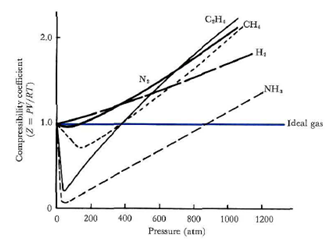
\includegraphics[scale=1.0]{R2.png}
\caption[Determinació de la constant dels gasos $R$]{R es pren com al valor límit de la fracció $\frac{P V_m}{T}$ per a tots els gasos: 
$R=\lim_{P \to 0} \frac{P V_{\rm m}}{T}= 0.08205 \frac{{\rm atm l}}{{\rm mol K}}$
}
\label{fig:R2}
\end{marginfigure}

\begin{exr}
    Quant gas hi ha en una mostra de volum 0.5 dm$^3$, a 80\si\degreeCelsius\ i 800 \si\torr\ de pressió?
    \end{exr}

       
    \begin{exr}
        Si a CN la densitat d'un gas ideal és de 1.62 g dm$^{-1}$, quina és la seva massa molar? i quina densitat tindrà a 300 K i 2.4$\times$10$^5$ Pa?
        \end{exr}

\subsection{Llei de Dalton}
La llei de les pressions parcials de Dalton estableix que la pressió total d'una mescla de gasos ideals és igual a la suma de les pressions parcials dels gasos individuals en la mescla. Matemàticament, es pot expressar així:

\[
P_{\text{total}} = P_1 + P_2 + P_3 + \cdots + P_n
\]

on \(P_{\text{total}}\) és la pressió total de la mescla, i \(P_1, P_2, \dots, P_n\) són les pressions parcials dels diferents gasos presents a la mescla.

La pressió parcial d'un gas és la pressió que exerciria aquest gas si ocupés tot el volum per si sol, a la mateixa temperatura.
  


\section{Teoria Cinètica dels Gasos}

Per tal de relacionar aquestes descobertes amb l'estructura atòmica de la matèria, ens cal introduir una teoria que representi els gasos de forma extremadament simple: un \textit{model}. En el nostre cas (veure Figura \ref{fig:TeoriaCinetica}),
\begin{itemize}
\item el gas és format per partícules que es comporten com a punts de massa, i
\item a més de no col·lidir, no exerceixen força les unes sobre les altres.
\end{itemize}
\begin{figure}[h]
\centering
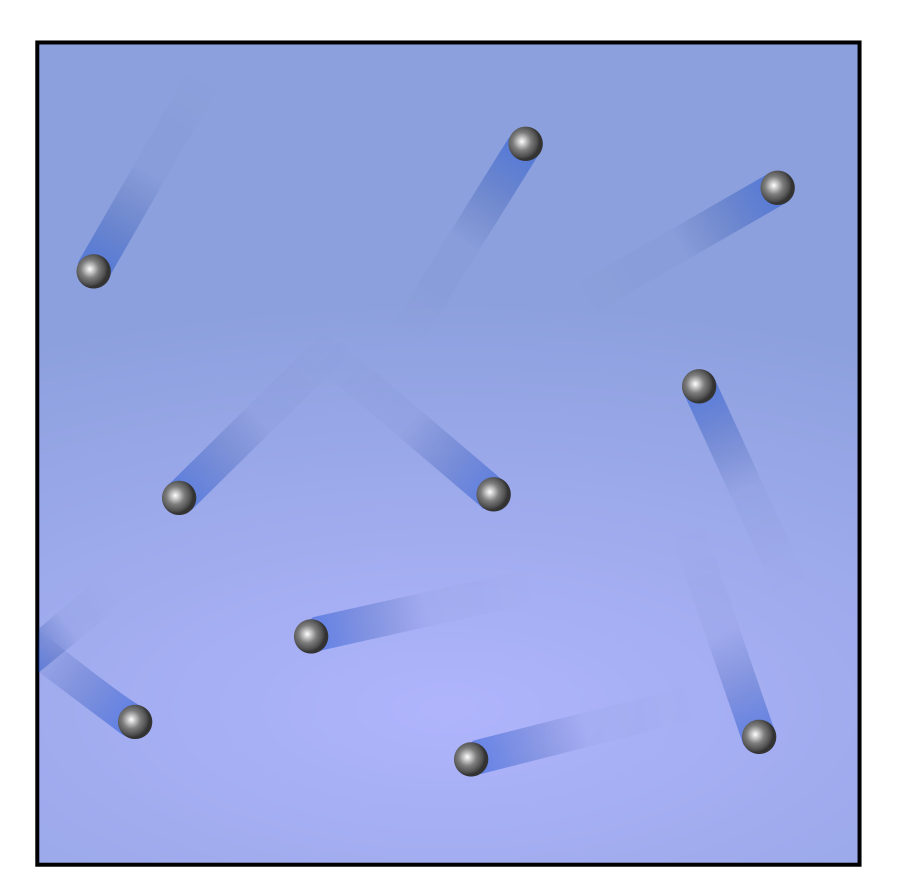
\includegraphics[scale=0.2]{TeoriaCinetica.png}
\caption{Representació del moviment de les partícules en un gas ideal.}
\label{fig:TeoriaCinetica}
\end{figure}
\begin{exr}
Pots calcular el volum ocupat per molècula en un gas ideal a CN?. Es troben dues molècules molt freqüentment en un gas a baixa pressió?
\end{exr}
Aquesta teoria, de forma relativament simple, ens permet expressar la pressió que s'exerceix sobre les parets d'un recipient per part del gas que conté segons:
\[
PV=\frac{2}{3} \left< E_c \right> = \frac{2}{3} N_0 \left< \frac{mc^2}{2} \right>
\]
on $N_0$ és el número d'Avogadro.

D'aquí s'extreuen resultats interessants, com que l'energia cinètica translacional d'un mol de gas és \[N_0 \frac{m <c^2>}{2}=\frac{3}{2} RT\] o bé, si dividim pel número d'Avogadro a esquerra i dreta obtenim la constant dels gasos per molècula a partir de l'energia cinètica per molècula (constant de Boltzmann $k$): 
\[\frac{m <c^2>}{2}=\frac{3}{2} kT\]
Aquest resultat ens diu que si dos gasos tenen la mateixa $T$, les seves molècules tenen la mateixa energia cinètica promig. 

\begin{exr}
Qui es mou més ràpid, una molècula d'oxigen o una de nitrogen en dues mostres d'aquests gasos a la mateixa temperatura? Pots explicar perquè la pressió és independent de la natura de les molècules?
\end{exr}

\begin{exr}
Calcula la velocitat mitjana de les molècules d'hidrògen a 25\si\degreeCelsius.
\end{exr}

La distribució de les velocitats de les partícules d'un gas segueix la distribució de Maxwell-Boltzmann\cite{mahan_quimica_1997}:
\[
\frac{\Delta N}{N}=4 \pi \left( \frac{m}{2 \pi kT}\right)^{3/2} \underbrace{e^{-mc^2/2kT}}_{\rm Boltzmann} c^2 \Delta c
\]
El factor de Boltzmann ens diu, en aquesta equació, que a qualsevol temperatura particular, acostuma a haver moltes menys molècules amb energies altes que amb energies baixes.
\begin{figure}[h]
\centering
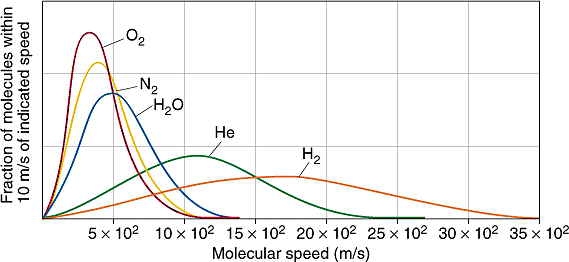
\includegraphics[scale=0.5]{BolzDist.png}
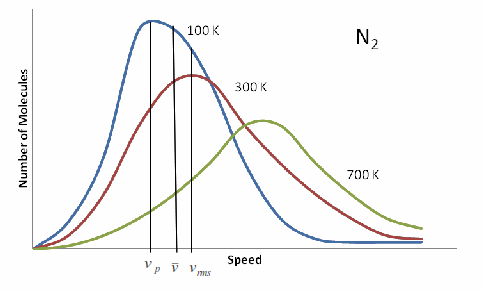
\includegraphics[scale=0.5]{MXDIST.png}
\caption{La distribució de Maxwell-Boltzmann per a diferents molècules i temperatures}
\label{fig:Maxwell}
\end{figure}






\subsection{Capacitat calorífica}

La capacitat calorífica d'una substància és la quantitat de calor en calories necessària per elevar 1\si\degreeCelsius\ la temperatura d'un gram de la substància.

De fet, això necessita precissió: no és el mateix fer aquest procés d'escalfament a volum constant que a pressió constant ($C_V$ vs $C_P$).

Si afegim calor a un gas, o bé s'expandeix (i per tant fa treball) o bé la velocitat de les seves particules augmenta.
A $V$ constant, l'escalfament produeix un increment d'energia cinètica:
\[\Delta E = \frac{3}{2} R \Delta T\]
però resulta que $\Delta E/ \Delta T$ és, justament, $C_V$ i, per tant, per a un gas monoatòmic ideal, $C_V=\frac{3}{2}R$ o, aproximadament, 3 cal/mol·grau.

En el cas de pressió constant, les partícules augmenten la seva energia cinètica i també exerceixen treball ($\Delta(PV)$):
\[\Delta(PV)=P\Delta V = P(V_2-V_1)=PV_2-PV_1\]
Per a un mol de gas, resulta que $PV=RT$ i, per tant, 
\[PV_2-PV_1=RT_2-RT_1=R\Delta T\]
Per tant, la capacitat calorífica extra pel fet de fer el procés a pressió constant és
\[\frac{\Delta (PV)}{\Delta T}=R\]
i, per tant, 
\[C_P=C_V+R 
=\frac{3}{2} R + R= \frac{5}{2}R\]
És fàcil veure que $C_P/C_V=5/3=1.67$ i podem comparar aquests coeficients per a diversos gasos reals, per tal d'establir diferències amb el seu comportament ideal (Taula \ref{tab:cpcv}).
\begin{margintable}
	\begin{center}
		\caption{Quocients de capacitat calorífica \cite{mahan_quimica_1997}.}
		\label{tab:cpcv}
		\begin{tabular}{cc|cc}
			\hline
			Gas & $C_P/C_V$ & Gas & $C_P/C_V$\\
			\hline
			He & 1.66 & \ch{H2} & 1.41 \\
			Ne & 1.66 & \ch{O2} & 1.40 \\
			Ar & 1.66 & \ch{N2} & 1.40 \\
			Kr & 1.66 & \ch{CO} & 1.40 \\
			Xe & 1.66 & \ch{NO} & 1.40 \\
			Hg & 1.66 & \ch{Cl2} & 1.36 \\
			\hline
		\end{tabular}
	\end{center}
\end{margintable}
\begin{exr}
Perquè hi ha aquestes diferències entre la columna de l'esquerra i la de la dreta de la Taula \ref{tab:cpcv}? (Adona't que si un gas monoatòmic ideal, pel fet d'estar només augmentant la seva energia cinètica translacional té una $C_V=\frac{3}{2}R$, es pot entendre que per a cada component (eix) necessita $\frac{1}{2}R$)
\end{exr}
\lct{
    Els quocients de la capacitat calorífica dels gasos diatòmics són molt menors que 1,67, i hem d'esbrinar la raó d'aquestes desviacions.

    Primerament, notem que $C_V$, la capacitat calorífica deguda al moviment de translació de les molècules, és igual a $\frac{3}{2}R$, i que hi ha tres components independents de velocitat associats amb el moviment de translació. Per tant, podem inferir que cadascun dels tres moviments de translació independents contribueix amb $\frac{1}{2}R$ a la capacitat calorífica molar. Sobre aquesta base, podríem esperar que, si algun altre tipus de moviment fos accessible a les molècules de gas, hi hauria més contribucions a la capacitat molar i aquestes entrarien en unitats de $\frac{1}{2}R$.
    
   A més de tenir els tres moviments de translació, una molècula diatòmica pot rotar al voltant del seu centre de massa segons dos modes mútuament perpendiculars i independents. Assignant $\frac{1}{2}R$ com la contribució de cadascun d'aquests moviments a la capacitat calorífica, tenim:
    
    \[
    C_V = \underbrace{\frac{3}{2}R}_{\text{traslació}} + \underbrace{\frac{1}{2}R + \frac{1}{2}R}_{\text{rotació}} = \frac{5}{2}R,
    \]
    
    \[
    C_P = C_V + R = \frac{7}{2}R,
    \]
    
    \[
    \frac{C_P}{C_V} = \frac{\frac{7}{2}R}{\frac{5}{2}R} = \frac{7}{5} = 1,40.
    \]
}




\subsection{Gasos no ideals}



En gasos reals, el factor de compressibilitat ve donat per
\[z=\frac{V_m}{V_{m,i}}=\frac{V_m}{RT/P}=\frac{PV_m}{RT}\]
no és 1, com succeiria a un gas ideal (veure Figura \ref{fig:FactorCompress}). En general, la desviació del comportament ideal esdevé més important quan el gas està més a prop d'un canvi de fase, com més baixa és la temperatura o com més alta és la pressió. 
\begin{figure}[h]
\centering
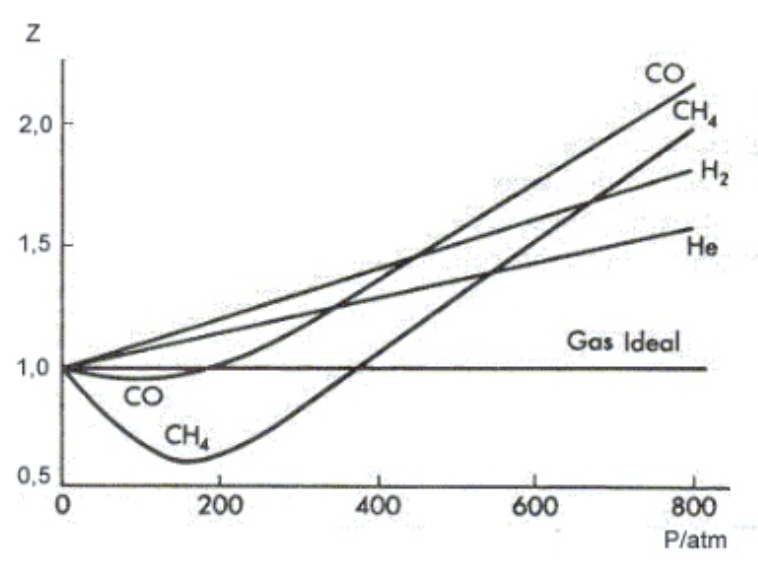
\includegraphics[scale=0.5]{FactorCompress.png}
\caption{Factor de compressibilitat per a diferents gasos a 0\si\degreeCelsius.}
\label{fig:FactorCompress}
\end{figure}

Per tal de millorar l'aproximació a la realitat podem considerar diferents aproximacions. 
En el desenvolupament de l'equació d'estat del gas ideal (EOS), es van fer dues hipòtesis:

\begin{itemize}
    \item El volum de les molècules de gas és insignificant en comparació amb el volum total i la distància entre les molècules.
    \item No existeixen forces atractives ni repulsives entre les molècules.
\end{itemize}

Van der Waals (1873) va intentar eliminar aquestes dues hipòtesis en el desenvolupament d'una equació empírica d'estat per a gasos reals. Per tal d'eliminar la primera hipòtesi, van der Waals va assenyalar que les molècules de gas ocupen una fracció significativa del volum a altes pressions i va proposar que el volum de les molècules, denotat pel paràmetre $b$, fos restat del volum molar real, $V$, en l'Eq. (5.45), per obtenir

\[
p = \frac{RT}{V - b}
\]

on el paràmetre $b$ és conegut com el covolum i es considera que reflecteix el volum de les molècules. La variable $V$ representa el volum real per mol de gas.

Segons això,
\[z=\frac{PV_m}{RT}=1+\frac{b}{RT}P\]
que té una forma lineal. Aixó explicaria el cas de la molècula d'hidrogen a la Figure \ref{fig:FactorCompress}.
Però què passa amb \ch{CH4} o \ch{CO}? Val la pena pensar que són molècules que es podran trobar líquides a temperatures més baixes amb major facilitat que no pas \ch{H2}. 
Per tal d'eliminar la segona hipòtesi, van der Waals va afegir un terme correctiu, denotat per $\frac{a}{V^2}$, a aquesta equació per tenir en compte les forces atractives entre les molècules.

Tenint en compte aquestes modificacions en la inclusió de $P$ i $V$ en l'equació des gasos ideals podem arribar (no ho fem aquí) a l'equació dels gasos ideals proposada per Johannes Diderick van der Waals el 1873:
\[
\left( P + \frac{a}{{V_m}^2} \right) (V_m -b)=RT
\]
o bé
\begin{equation}
\left( P + \frac{n^2 a}{V^2} \right) (V -nb)=nRT
\label{Eq:vdW}
\end{equation}

\begin{exr}
Què passa segons l'Equació \ref{Eq:vdW} si la pressió es fa propera a zero o bé la temperatura es fa molt gran per a un gas real?   La figura mostra el factor de compressibilitat per a un mateix gas a diferents temperatures
\begin{center}        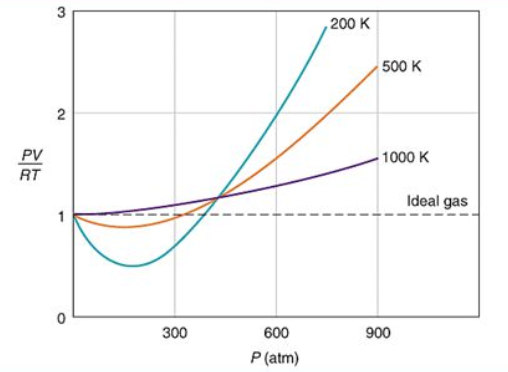
\includegraphics[scale=1.0]{FactorCompressT.png}
\end{center}
\end{exr}


Les forces de van der Waals que fan que es perdi la idealitat són degudes a tres contribucions:
\begin{enumerate}
\item Efecte d'orientació: forces dipol-dipol.
\item Efecte de distorsió: forces d'inducció.
\item Efecte de dispersió: forces de dispersió.
\end{enumerate}

\begin{exr}
Perquè \ch{CO2} i \ch{O2} tenen una desviació negativa respecte al comportament del gas ideal a pressions i temperatures moderades, mentres que l'He i el \ch{H2} presenten una deviació positiva en les mateixes condicions?
\end{exr}

\newpage
\section{Codis}

\begin{lstlisting}[language=Matlab, caption={Codi Matlab per dibuixar una distribució de Maxwell-Boltzmann}]
    clc; clear; close all;
    
    % Definim constants
    kB = 1.38e-23;  % Constant de Boltzmann (J/K)
    T = 300;        % Temperatura en Kelvin
    m = 4.65e-26;   % Massa de la molècula (kg) (exemple: molècula de nitrogen)
    
    % Definim el rang de velocitats
    v = linspace(0, 2000, 1000);  % Rang de velocitats (m/s)
    
    % Funció de distribució de Maxwell-Boltzmann
    f_v = ( (m / (2 * pi * kB * T))^(3/2) ) * 4 * pi * v.^2 .* exp(-m * v.^2 / (2 * kB * T));
    
    % Representació gràfica de la distribució
    figure;
    plot(v, f_v, 'b', 'LineWidth', 2);
    xlabel('Velocitat (m/s)');
    ylabel('Densitat de probabilitat f(v)');
    title('Distribució de Maxwell-Boltzmann');
    grid on;
    
    % Càlcul de la velocitat més probable, la velocitat mitjana i la velocitat quadràtica mitjana
    v_mp = sqrt(2 * kB * T / m);  % Velocitat més probable
    v_mitjana = sqrt(8 * kB * T / (pi * m));  % Velocitat mitjana
    v_rms = sqrt(3 * kB * T / m);  % Velocitat quadràtica mitjana
    
    hold on;
    xline(v_mp, '--r', 'Velocitat més probable', 'LabelHorizontalAlignment', 'right');
    xline(v_mitjana, '--g', 'Velocitat mitjana', 'LabelHorizontalAlignment', 'right');
    xline(v_rms, '--m', 'Velocitat RMS', 'LabelHorizontalAlignment', 'right');
    legend('Distribució de Maxwell-Boltzmann', 'Velocitat més probable', 'Velocitat mitjana', 'Velocitat RMS');
    hold off;
    \end{lstlisting}